\documentclass[conference]{IEEEtran}
\IEEEoverridecommandlockouts
% The preceding line is only needed to identify funding in the first footnote. If that is unneeded, please comment it out.
\usepackage{cite}
\usepackage{amsmath,amssymb,amsfonts}
\usepackage{algorithmic}
\usepackage{graphicx}
\usepackage{textcomp}
\usepackage{xcolor}
\def\BibTeX{{\rm B\kern-.05em{\sc i\kern-.025em b}\kern-.08em
    T\kern-.1667em\lower.7ex\hbox{E}\kern-.125emX}}
\begin{document}

\title{A Survey on Multi-modal Emotion Detection Techniques\\

}

\author{\IEEEauthorblockN{1\textsuperscript{st} Nihir}
\IEEEauthorblockA{\textit{dept. name of organization (of Aff.)} \\
\textit{name of organization (of Aff.)}\\
City, Country \\
email address or ORCID}
\and
\IEEEauthorblockN{2\textsuperscript{nd} Given Name Surname}
\IEEEauthorblockA{\textit{dept. name of organization (of Aff.)} \\
\textit{name of organization (of Aff.)}\\
City, Country \\
email address or ORCID}
}

\maketitle

\begin{abstract}
This document is a model and instructions for \LaTeX.
This and the IEEEtran.cls file define the components of your paper [title, text, heads, etc.]. *CRITICAL: Do Not Use Symbols, Special Characters, Footnotes, 
or Math in Paper Title or Abstract.
\end{abstract}

\begin{IEEEkeywords}
component, formatting, style, styling, insert
\end{IEEEkeywords}

\section{Introduction}
Multimodal emotion detection in machine learning refers to the task of recognizing and understanding human emotions by using multiple sources of data or modalities. \cite{hina2022multimodal}
The modalities can  be provided in various ways such analysing the text, audios, videos, images, Physiological Signals and many more.

Machine learning techniques used in multimodal emotion detection include fusion methods, where information from different modalities is combined into a unified representation, and multi modal deep learning models, which integrate various types of neural networks to process different modalities simultaneously \cite{joshi2022cogmen}. For integrating information from various sources, multimodal deep learning architectures that can handle inputs from several modalities are used. These could include parallel CNNs, RNNs, or transformers for several modalities, followed by multimodal fusion layers \cite{sharafi2022novel}. 

\begin{figure}[htbp]
\centerline{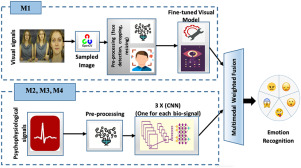
\includegraphics{Multimodal.png}}
\caption{Multimodal Classification for Emotion Detection.\cite{KUMAR2022104483}}
\label{fig}
\end{figure}

The initial stage in multimodal emotion identification is to efficiently fuse information from diverse modalities. Merge the raw data from all modes into a single input representation. Combining text embeddings, audio features, and image features. Textual data can be processed using Recurrent Neural Networks (RNNs), Long Short-Term Memory (LSTM) networks, or Transformers. Convolutional Neural Networks (CNNs) or Recurrent Neural Networks (RNNs) are neural networks that are used to process audio signals or spectrogram images. Convolutional Neural Networks (CNNs) like ResNet or VGG are used to process pictures or video frames \cite{huang2019multimodal}.

\section{Types of Data in Emotion Detection}

Facial emotion detection using images is a technology that involves analyzing facial expressions in images or videos to determine the emotions being displayed by individuals. The first step is to identify and locate the faces within the image. This is often done using techniques like Haar cascades, deep learning-based methods (e.g., Convolutional Neural Networks or CNNs), or other advanced computer vision algorithms.  Once faces are detected, relevant features are extracted from the face regions. After extracting features, machine learning techniques are employed to classify the detected emotions. Various algorithms can be used for this, such as Support Vector Machines (SVMs), Random Forests, or more commonly, deep learning models like CNNs.

Emotion detection using voice, also known as speech emotion recognition, is another fascinating application of machine learning. Choose a suitable machine learning model for emotion detection. Recurrent Neural Networks (RNNs), Convolutional Neural Networks (CNNs), and more advanced models like Long Short-Term Memory (LSTM) networks or Gated Recurrent Units (GRUs) are commonly used for sequential data like audio.

Emotion detection using video data involves analyzing facial expressions and other visual cues to infer the emotional state of individuals. Detect and track faces within each video frame. This can be achieved using techniques like Haar cascades, deep learning-based object detection models (e.g., Faster R-CNN, SSD), or facial landmark detection models.

\begin{figure}[htbp]
\centerline{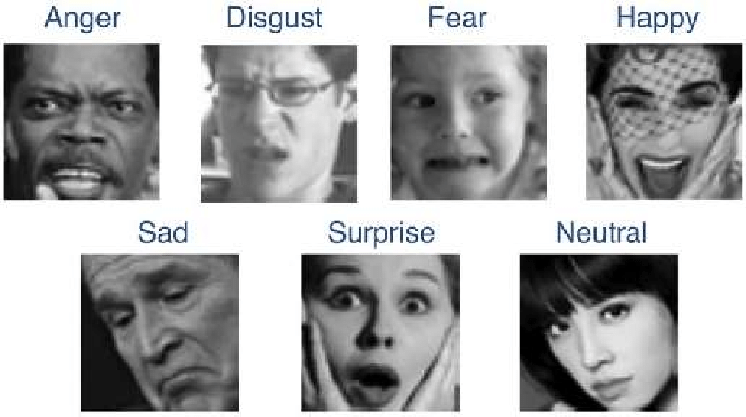
\includegraphics[scale=0.35]{Facial_Emotion.png}}
\caption{Facial Emotion.}
\label{fig}
\end{figure}

Emotion detection using voice, also known as speech emotion recognition, involves analyzing audio signals (such as spoken words or speech segments) to determine the emotional state of the speaker.  The first step is to extract relevant features from the audio signal. These features can include acoustic characteristics such as pitch, intensity, rhythm, spectral content, and more. These features capture the patterns and nuances in the voice that are associated with different emotions. After extracting features, machine learning techniques are used to classify the detected emotions. Similar to facial emotion detection, algorithms like Support Vector Machines (SVMs), Random Forests, and deep learning models are commonly employed for this task \cite{s19122730}.

MFCCs are commonly used features for speech processing tasks. They capture the spectral characteristics of the voice signal and have been successful in representing emotional information.

Emotion detection from voice can be challenging due to factors like variations in accents, speech rate, background noise, and individual differences in speech patterns. Robustness to these factors requires careful data preprocessing, feature engineering, and model design. To improve the model's performance over time, you can collect user feedback and retrain the model with additional data. This can help the model adapt to different user preferences and variations.

\section{Techniques Used}

\subsection{Deep Learning techniques used for Emotion Detection}

Transformers are one of the techniques used in the Deep learning framework. The textual data can be processed by the transformers for recognizing the emotions \cite{karatay2022multi},\cite{le2023multi}. 
Transformers are used in sequence transduction. This means that if we want to transform any input sequence to the output sequence, we can use transformers. The applications of transformers include Speech recognizing, text recognition and many more. When the speech is converted into sequence of words, it is given as an input to the transformer. The architecture detects the speech by extracting its features and output of sequence is produced from the transformers. The model attends to all the other words in the sentence and calculates a weighted sum of their representations to create the output representation for each word. it first encode the input sequence into vector representation. This step is called as Encoding \cite{huang2020multimodal}.
To process the input and output sequences, the decoder employs self-attention and cross-attention techniques. Transformers are typically trained using supervised learning with large labeled data sets. After each layer, layer normalization and residual connections are applied. Layer normalization aids in training process stability, while residual connections allow gradients to flow more effectively through the network, eliminating disappearing gradients and making deep models easier to train.\cite{lian2021ctnet} 

\begin{figure}
\centerline{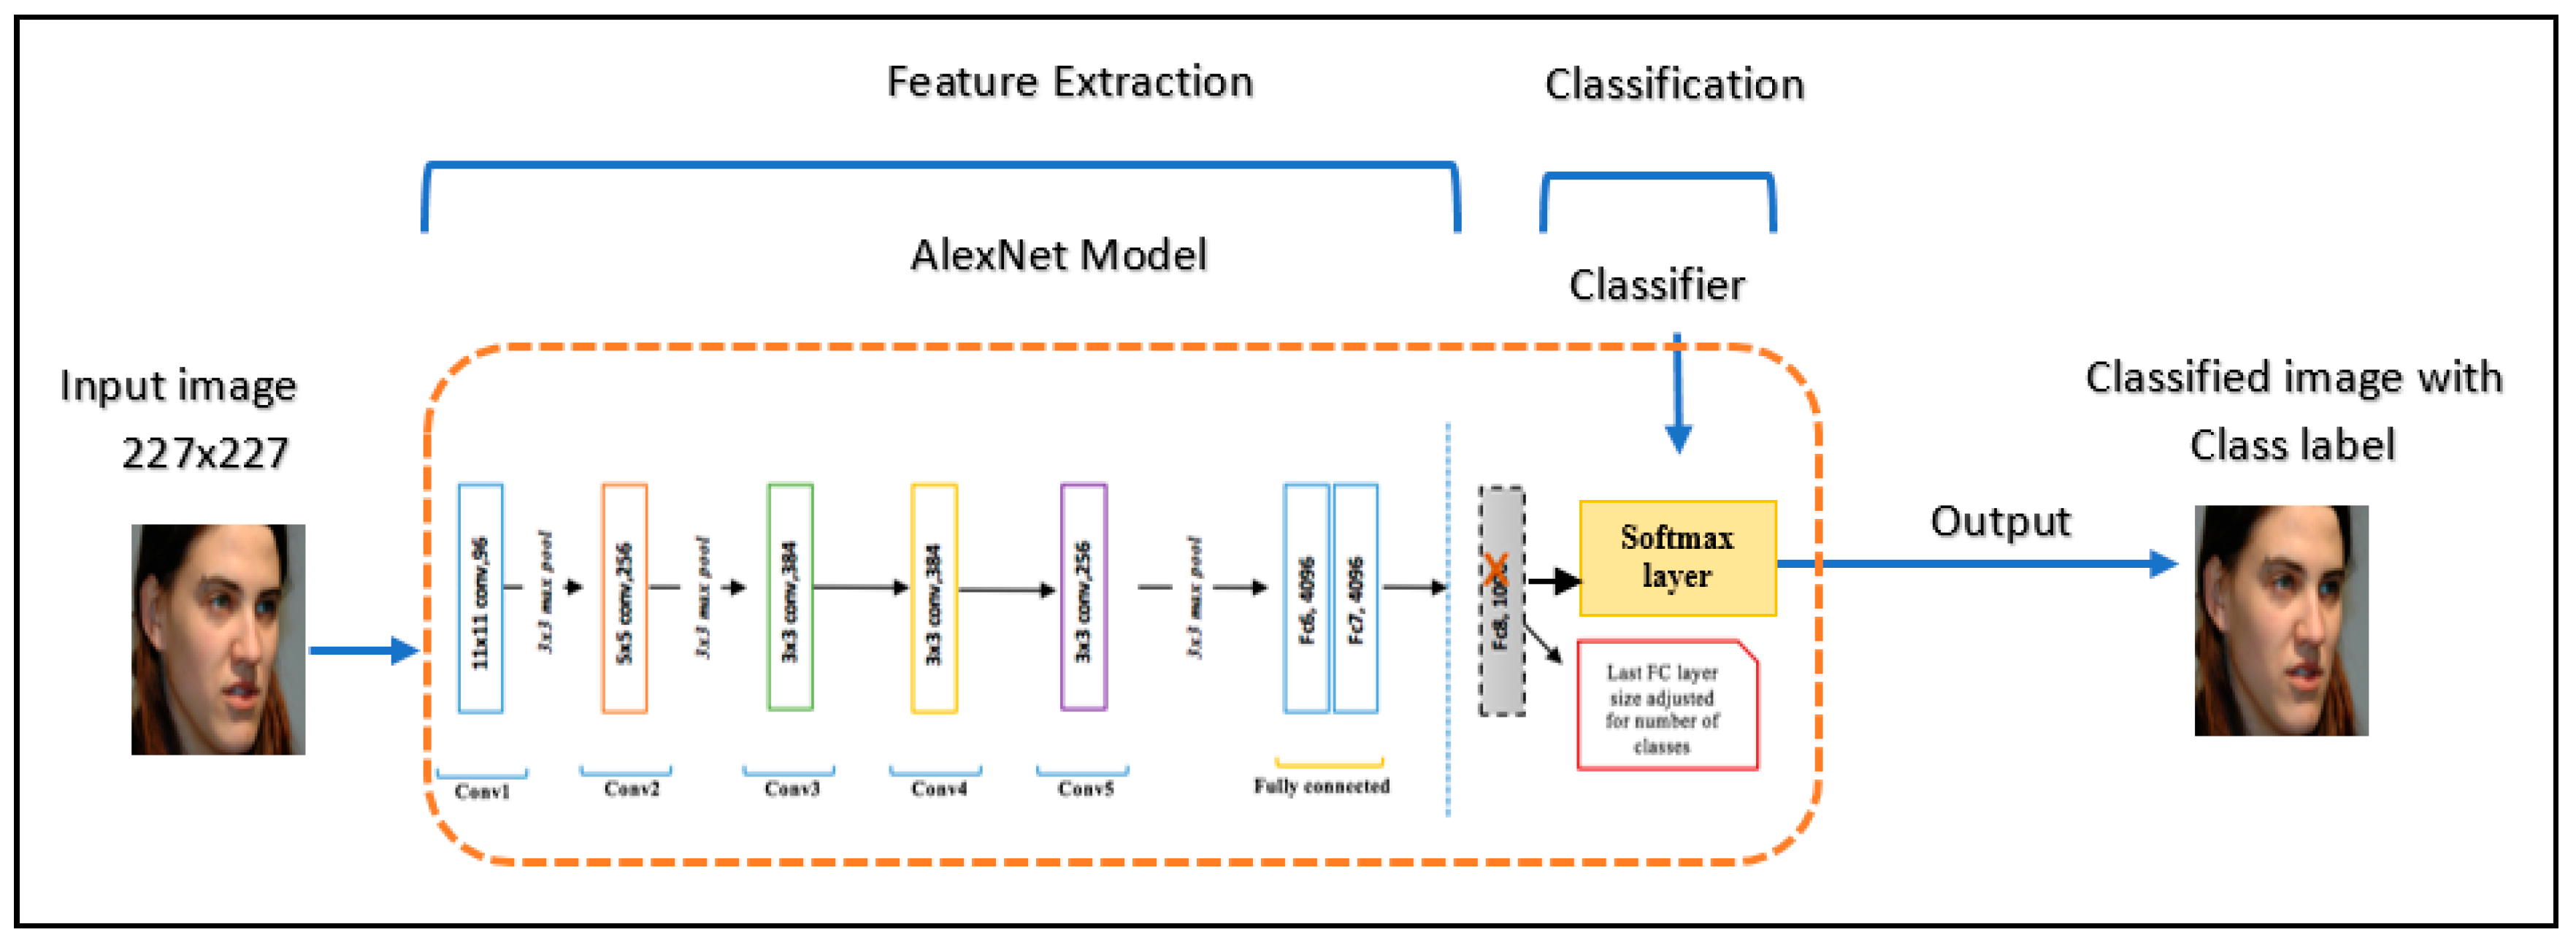
\includegraphics[scale=0.07]{DNNmodel.png}}
\caption{DNN Model \cite{app9204397}}
\end{figure}


GANs can be used for generating realistic data samples in one modality based on the information from other modalities \cite{vidal2023multimodal}, \cite{luo2019gan}. 
Another technique is the Transfer learning. It is the concept in which once the machine learning model has been trained to get the patterns out of the data, the concept of transfer process is used. n the context of emotion detection, transfer learning can be employed to leverage pre-trained models that have been trained on large datasets for tasks like sentiment analysis, language understanding, or image recognition. This approach helps improve the performance of emotion detection models, especially when limited labeled data is available for the specific emotion detection task. This utilizes the information from the trained model to improve its accuracy and is able to perform the task which is relevant to the previous one without training the model. Basically, it is the pre-trained model that can be reused for solving another problem. The BERT model of transfer learning can be used for the text recognition \cite{padi2022multimodal}. 
The Ensemble learning approach of Combining multiple deep learning models, each specialized in a specific modality, can lead to improved performance \cite{salama20213d}. 
Fusion CNNs models can be used to  to combine information from multiple modalities at various levels \cite{zhang2021multimodal}.  Ensemble models combine predictions from multiple individual models to improve overall performance. You can create an ensemble of GRU-based models with different hyperparameters, input representations, or initializations to improve the diversity of predictions and enhance emotion detection accuracy.
Multimodal Attention Mechanisms allow the model to focus on the most relevant parts of each modality when making predictions. Selective fusion of data from several modalities is possible with multimodal attention \cite{zhang2023multimodal}.While not GRUs, TCNs are an alternative architecture for sequence modeling that can be used for emotion detection. TCNs use dilated convolutions to capture long-range dependencies in sequences, making them suitable for tasks where context over longer distances is crucial.
TCNs often use residual connections to mitigate the vanishing gradient problem and improve training stability. Residual connections enable the network to directly learn the residual (difference) between the input and the output of a layer. This facilitates the training of deeper networks. After applying convolutional layers, TCNs often use temporal pooling layers (e.g., max pooling) to downsample the sequence. This helps in reducing the computational complexity and capturing higher-level features. Following the convolutional and pooling layers, TCNs typically have one or more fully connected layers that perform the final classification for emotion detection. These layers aggregate the features learned by the convolutional layers and make predictions based on the context captured in the sequence \cite{zheng2023two}. The final output layer of a TCN is usually a softmax layer that assigns a probability distribution over the emotion classes. This allows the network to make emotion predictions based on the learned features. Ns are trained using backpropagation and gradient descent, just like other neural network architectures. The loss function used for training depends on the task, but for emotion detection, it could be categorical cross-entropy \cite{hu2023multiscale}. During training, the network learns to adjust its parameters to minimize the difference between predicted and actual emotion labels. The advantages of TCNs for emotion detection include their ability to capture long-range dependencies in sequences, their parallel processing of different features, and their potential to handle variable-length sequences. However, like any neural network architecture, the effectiveness of TCNs depends on factors such as the quality and size of the training data, the architecture's hyperparameters, and the task's inherent complexity.

 NLP techniques, such as word embeddings (Word2Vec, GloVe) and recurrent neural networks (RNNs), are used to capture semantic relationships and context in text, aiding emotion detection.
 Electroencephalogram (EEG) signals are analyzed to identify patterns that correspond to emotional states. Machine learning models classify these patterns to detect emotions. Mel-Frequency Cepstral Coefficients (MFCCs) are a common feature extraction technique for speech signals that captures relevant spectral characteristics for emotion recognition.

\begin{figure}[htbp]
\centerline{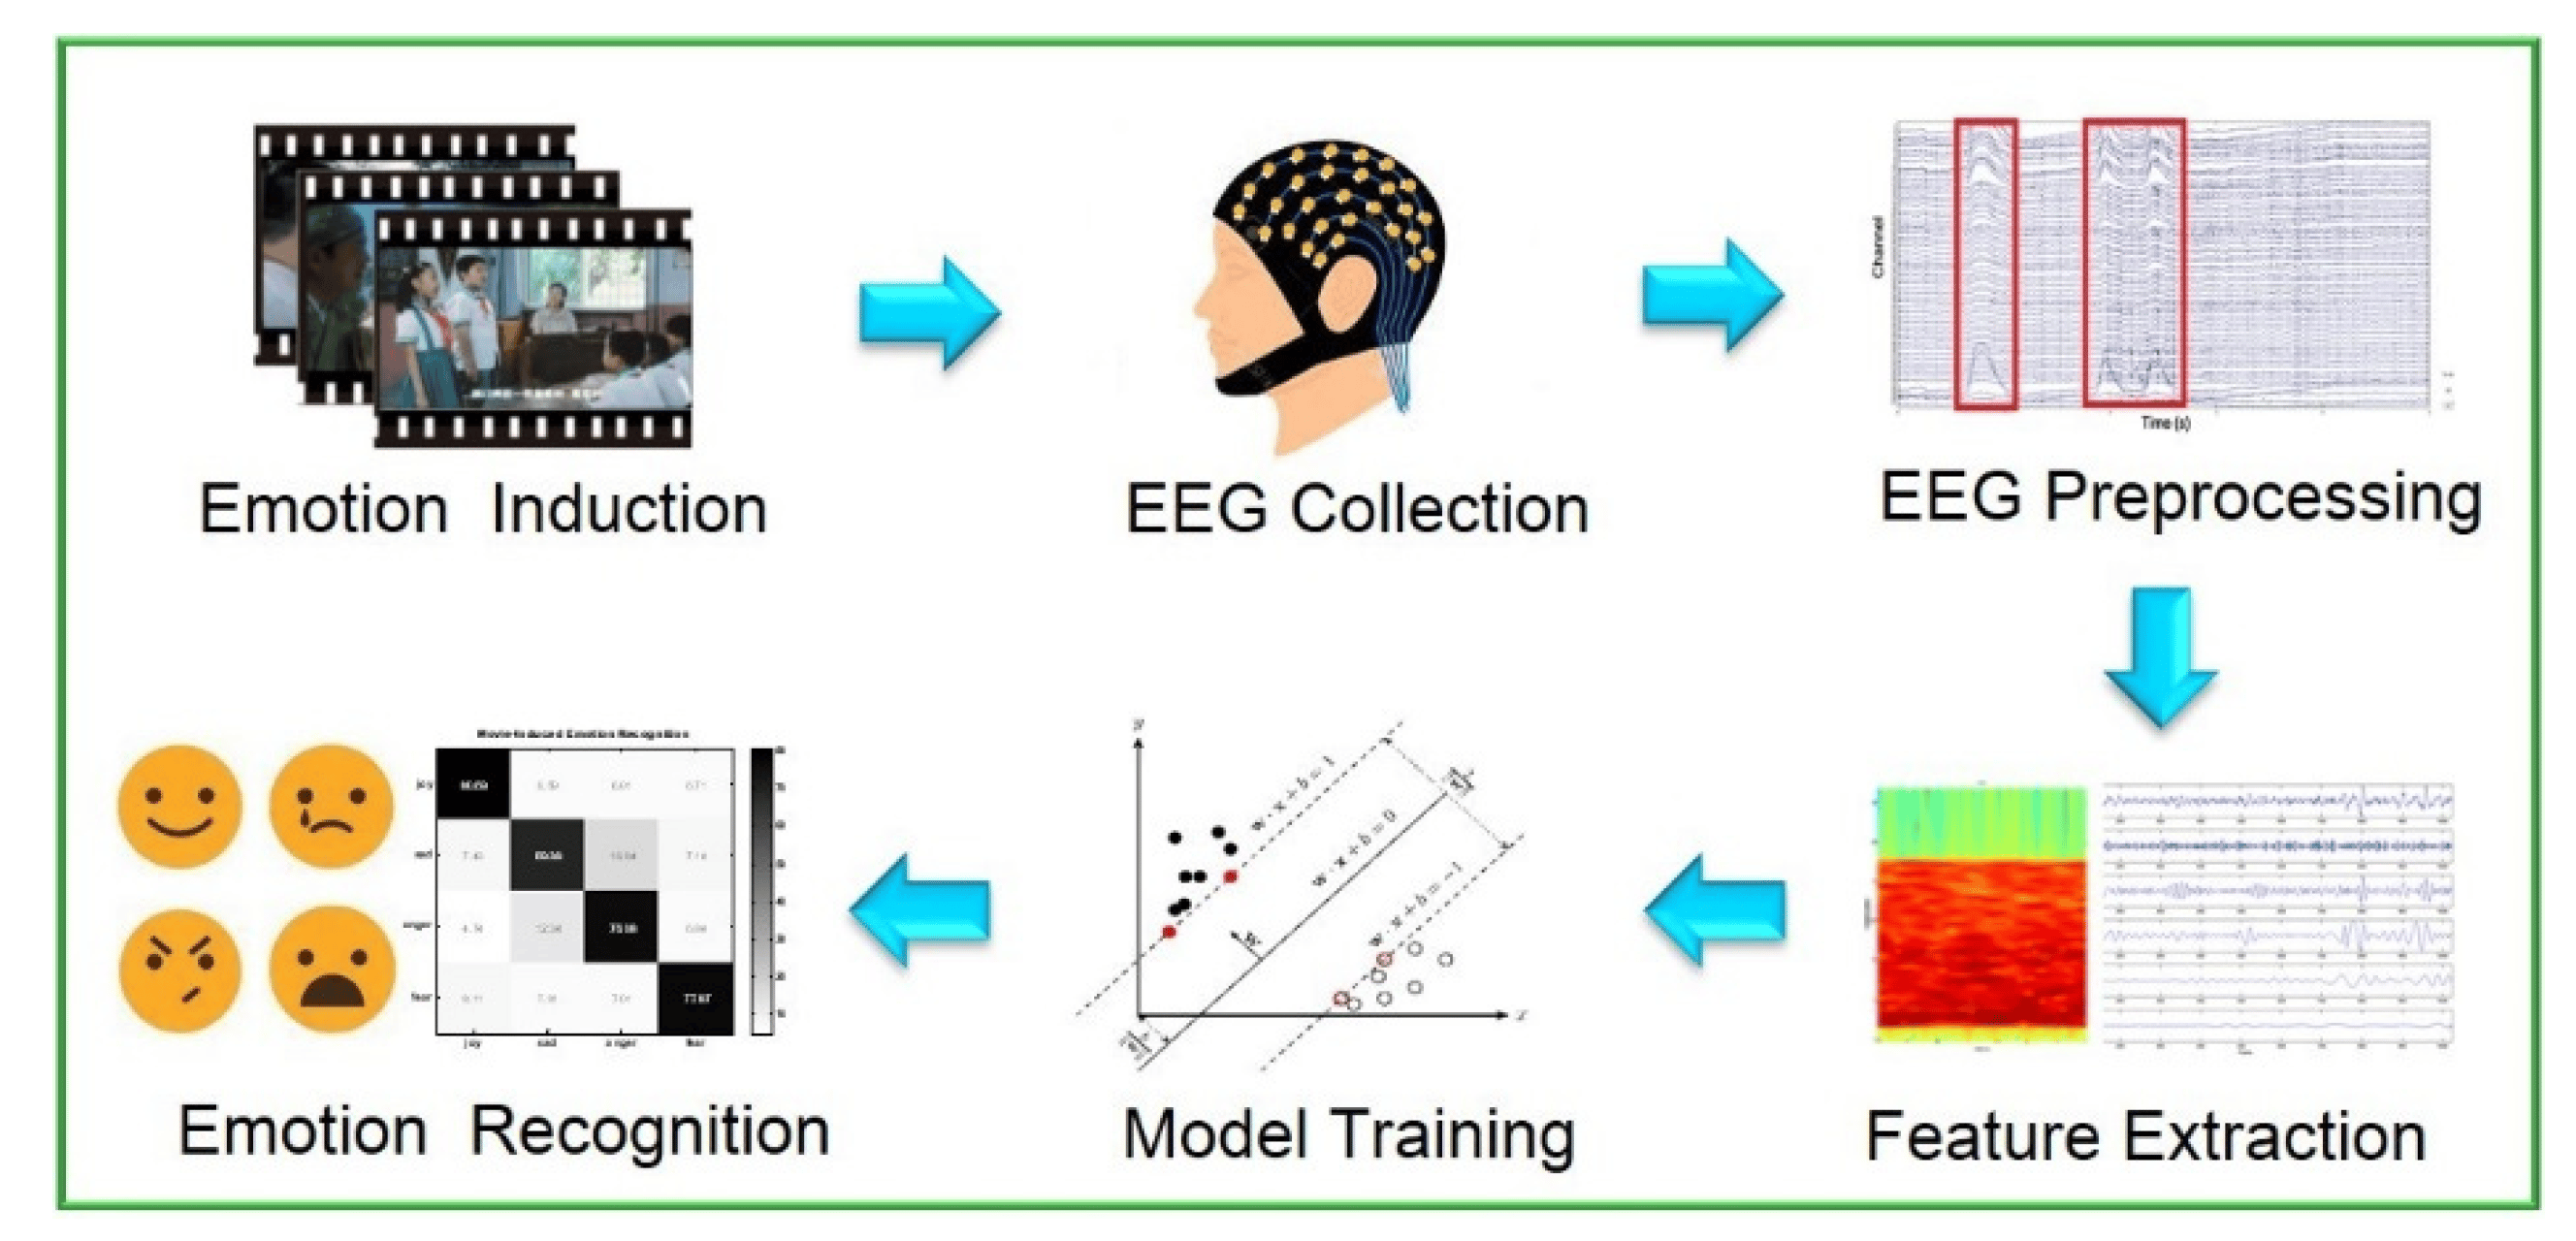
\includegraphics[scale=0.07]{EEG.png}} 
\caption{Emotion detection using EEG  \cite{zheng2023two}}
\label{fig}
\end{figure}
\cite{ma2022data}
EEG measures the electrical activity of the brain by placing electrodes on the scalp. EEG signals are recorded over time, resulting in a time-series data format. Participants are often exposed to stimuli that evoke different emotional responses, and their brain activity is recorded during these stimuli presentations. EEG signals are raw and complex time-series data. To make them suitable for machine learning algorithms, relevant features need to be extracted. Features can include spectral power, frequency bands (such as alpha, beta, theta), connectivity measures (like coherence or phase synchronization), and statistical features. These features capture different aspects of brain activity related to emotions. EEG data can be high-dimensional due to the large number of electrodes. Dimensionality reduction techniques like Principal Component Analysis (PCA) or feature selection methods are often applied to reduce the number of features and maintain only the most informative ones. Various machine learning and deep learning models can be used to predict emotions from EEG features. Some common models include Support Vector Machines (SVMs), Random Forests, Recurrent Neural Networks (RNNs), Convolutional Neural Networks (CNNs), and Long Short-Term Memory (LSTM) networks. The selected model is trained on labeled EEG data, where each sample is associated with an emotional label (such as happiness, sadness, anger, etc.). The model learns to map the extracted EEG features to the corresponding emotional states. The trained model is validated on a separate dataset that it hasn't seen during training. This helps assess the model's generalization ability and identify potential overfitting. Testing is then conducted on a completely unseen dataset to evaluate its performance in real-world scenarios. Once trained and validated, the EEG model can take new EEG data as input and predict the associated emotional state. The model's output could be a probability distribution over different emotions or a single predicted emotion label.

\section{Related Works}

The \cite{siriwardhana2020multimodal} shows the working of transformer self attention based architecture. \cite{makiuchi2021multimodal} shows the fusion of multimodal architecture, which ultimately provides higher accuracy with better results. \cite{ju2020transformer} positional encoding is added to the input embeddings to provide information about the word's position in the input sequence.
The accuracy of time-contextual learning's video emotion recognition can be increased with the use of an entirely novel network initialization technique.  A video multimodal emotion identification system based on an attention fusion network is suggested in order to get around the weight consistency of each modality in multi modal fusion \cite{huan2021video},\cite{abdullah2021multimodal}.

\begin{figure}[htbp]
\centerline{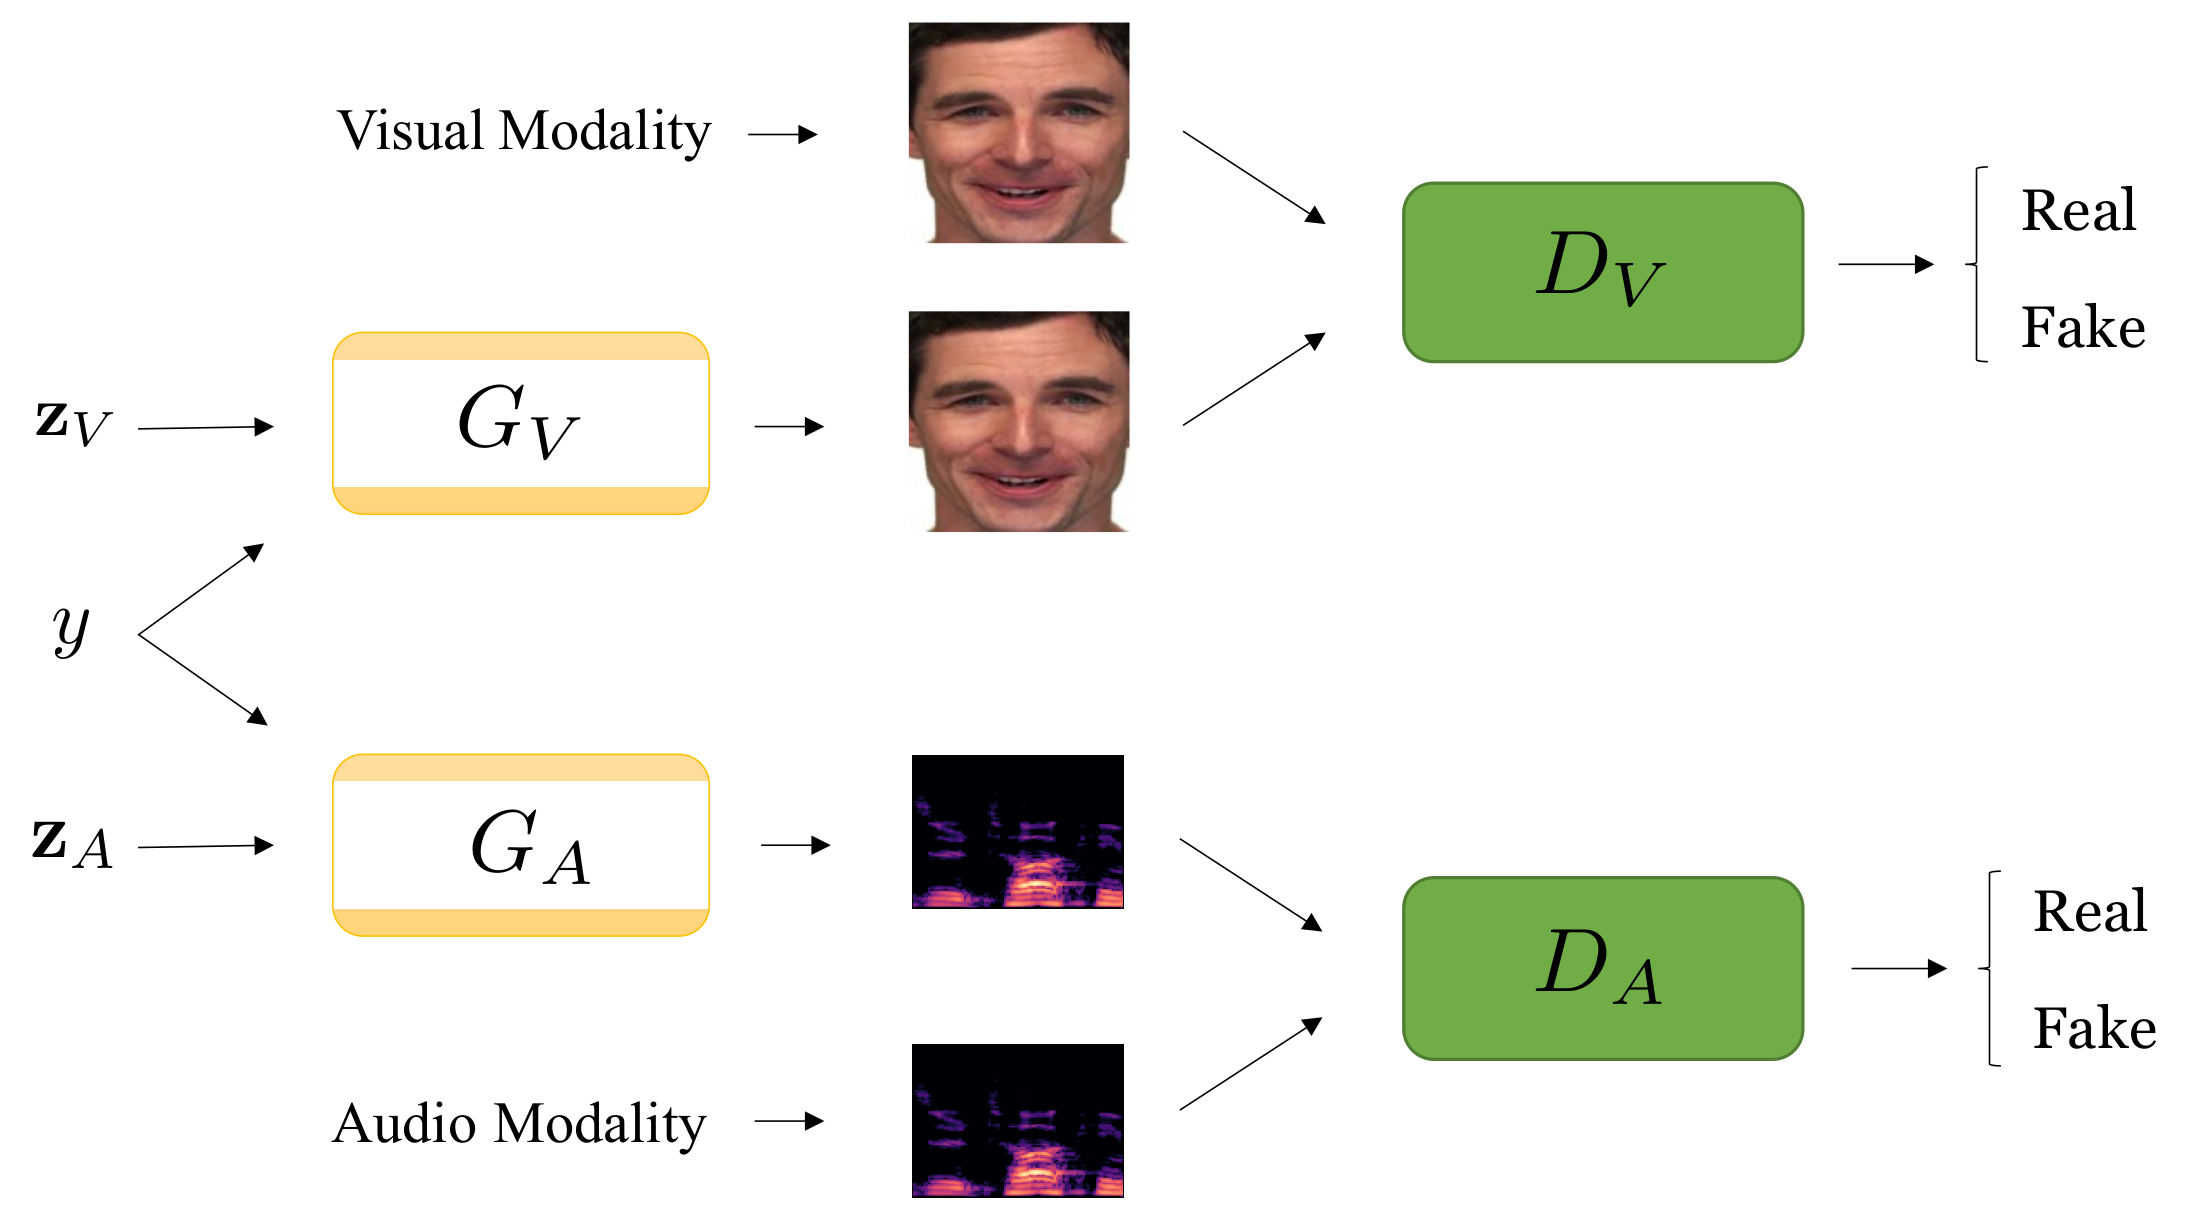
\includegraphics{GANs.png}}
\caption{Emotion detection using GANs \cite{KUMAR2022104483}}
\label{fig}
\end{figure}
\cite{ma2022data}

GAN stands for "Generative Adversarial Network," and it is a powerful framework in deep learning for generating new data that is similar to existing data. GANs consist of two neural networks, a generator and a discriminator, which are trained simultaneously through a competitive process. GANs can be used for image-to-image translation challenges when the emotion detection model benefits from having several visual representations of emotions. \cite{sharafi2022novel} GANs, can transform an image of a person's facial expression into different emotional expressions, resulting in a more diversified set of data for training the emotion recognition model. GANs can be used to produce visuals based on certain emotions. GANs can supplement training data for emotion detection models. GANs can assist increase the variety of the dataset by generating more synthetic samples, which can lead to better generalization and increased performance of the emotion detection model\cite{setyono2023data}. Sima et. al \cite{das2023emotion} had reviwed various advantages and disadvantages of GAN architecture for emotion detection.

\begin{figure}
\centerline{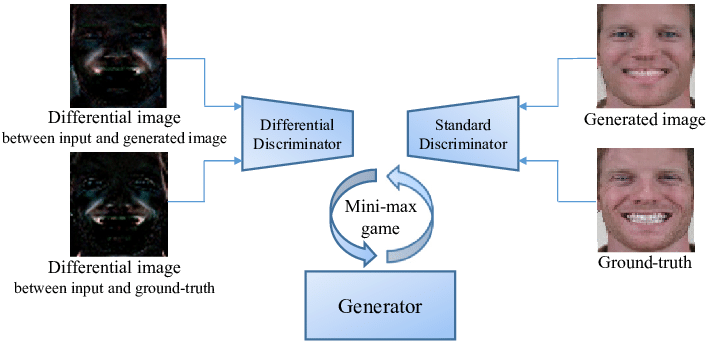
\includegraphics[scale=0.3]{GAN.png}}
\caption{GAN architecture for emotion detection \cite{article}}
\end{figure}

\cite{aldawsari2023optimizing} presented specialized EEG channel and feature selection techniques to exclude extraneous data from high-quality features. Haya et. al \cite{hasnul2023augmenting} presented The classification accuracy of five machine learning algorithms—the k-nearest neighbors (KNN), support vector machine, decision tree, random forest, and multilayer perceptron—is used to evaluate augmentation strategies. Mohan Karnati et. al \cite{karnati2023understanding} presented the survey for facial expression recognition (FER).

Gated Recurrent Unit (GRU) networks, like other recurrent neural networks (RNNs), can be used for emotion detection tasks, particularly when dealing with sequential data such as text or speech. GRUs are a form of RNN that overcomes some of the drawbacks of traditional RNNs, such as the vanishing gradient problem, which can make it difficult for the model to capture long-term dependencies in sequences \cite{maji2023multimodal}.


Bubai et. al \cite{electronics11091328} presented Mel-spectrograms  using the Conv-Cap module, and the remaining spectral characteristics from the input tensor were obtained using the Bi-GRU. Each module made use of the self-attention layer to identify the attention weight and preferentially concentrate on the best cues in order to produce high-level features. 
\begin{figure}
\centerline{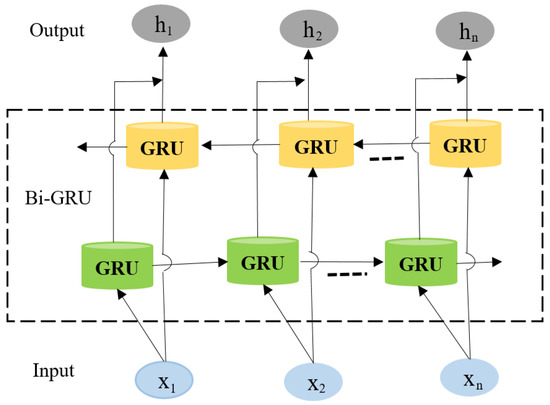
\includegraphics[scale=0.5]{GRU.png}}
\caption{GRU architecture for emotion detection \cite{electronics11091328}}
\end{figure}
 With the aid of six bidirectional gated recurrent units and two convolution layers (MBi-GRUMCONV), the model performs sentiment classification on vectorized reviews using two Word2Vec algorithms, namely the Skip Gram and Continuous Bag of Words, in three distinct vector sizes (100, 200, and 300) \cite{bacsarslan2023mbi}. \cite{han2023speech} A deep residual shrinkage network with bi-directional gated recurrent unit (DRSN-BiGRU) was proposed. A speaker emotion detection unit (SED-Unit), and a decoder with speaker emotion detection Bi-LSTM (SED-Bi-LSTM) was proposed \cite{liang2023mmateric}. In a bidirectional GRU, the input sequence is processed in both directions, forward and backward. This enables the model to capture information from both past and future contexts. Bidirectional GRUs are particularly useful for emotion detection tasks as they allow the model to understand the context surrounding each word in the sequence.

This research presents a novel emotion recognition system based on various modalities, such as electroencephalogram (EEG), galvanic skin response (GSR), and facial expressions \cite{cimtay2020cross},\cite{chowdary2022emotion}. In this concept, for each modality, a dedicated neural network is constructed to process the respective data \cite{liu2023multi}. The data is processed by modality-specific networks, and the features that were extracted are then integrated to produce a combined representation. \cite{priyadarshini2023emotion}, \cite{pan2023multimodal}
The hybrid LSTM/CNN model is used in this investigation. \cite{zhang2021multimodal},\cite{tzirakis2017end}. In order to improve the precision of feature extraction, the spatial and temporal features derived from video frames are fused together \cite{sharafi2022novel},\cite{gu2021multimodal}. Yun Gu et. al \cite{gu2023domain} presemted EEG model  for the intelligence and humanization of brain-computer interface (BCI). \cite{vempati2023systematic} presented a review on Brain-Computer Interaction (BCI) system intelligence has become more dependent on electroencephalogram (EEG)-based emotion recognition. 30 hearing-impaired participants who were watching video clips showcasing six different emotions—happiness, inspiration, neutral, anger, fear, and sadness—were asked to record their EEG activity in \cite{bai2023sect}

Hybrid neural network architecture was designed by U.M.Fernandes Dimlo et. al \cite{dimlo2023innovative}.

Transformers: \cite{nagarajan2023emotion} showed Emotion Recognition from Videos Using Transformer Models. \cite{le2023multi} presented transformer-based fusion and representation learning method to fuse and
enrich multimodal features from raw videos for the task of multi-label video emotion recognition. \cite{hsu2023applying} presented bi-modal transformer. \cite{wu2023transformer}  A large-scale self-collected physiological dataset was used to pre-train the SSL model, and three publicly available supervised emotion detection datasets were used to freeze or fine-tune the resultant encoder. \cite{kumar2023emotion} Word embedding is used to compare various machine learning and deep learning algorithms and show accuracy.

Transfer Learning: \cite{shehada2023lightweight} uggested to use a unique model that transfers features between datasets. With the help of this model, it is possible to apply characteristics discovered while resolving a limited number of challenging new situations. 


\section{Discussions}
The challenges in multimodal emotion detection include aligning data from different modalities.
Since emotions are very context-dependent, it is essential to accurately capture the context during emotion detection. Contextual data integration across several modalities is still an unsolved research issue.
Handling missing or noisy information, and designing effective fusion strategies to combine the modalities appropriately may be a challenging task to perform. \cite{liang2020semi}
Considerations for Multilingualism and Diversity Cultural and linguistic obstacles can affect how emotions are communicated and understood. Building models with universal applicability requires research into understanding and overcoming these differences.
While categorizing fundamental emotions (such as happiness and sorrow) is a common topic of current study, measuring the level of intensity or valence of emotions is still a difficult task.
Collecting accurate and reliable labeled data for training emotion detection models can be difficult. Emotions are often subtle and can be influenced by various contextual factors, making it challenging to determine the true emotional state of an individual.

Emotions can be expressed in various ways, and individuals may express the same emotion differently. Emotions are influenced by the context of the speech, and the same words spoken in different contexts can convey different emotions. Background noise and other acoustic disturbances can affect the accuracy of emotion detection. Collecting large and diverse emotion-labeled audio datasets can be challenging.

\cite{jia2022multimodal} GRU networks have the advantage of capturing long-term dependencies in sequential data. The GRU's update and reset gates enable it to manage the flow of information over time. The update gate aids valuable information from the previous time step, whereas the reset gate regulates how much historical information is forgotten. This gating mechanism allows GRU networks to learn patterns and dependencies across lengthy sequences.

\begin{figure}
\centerline{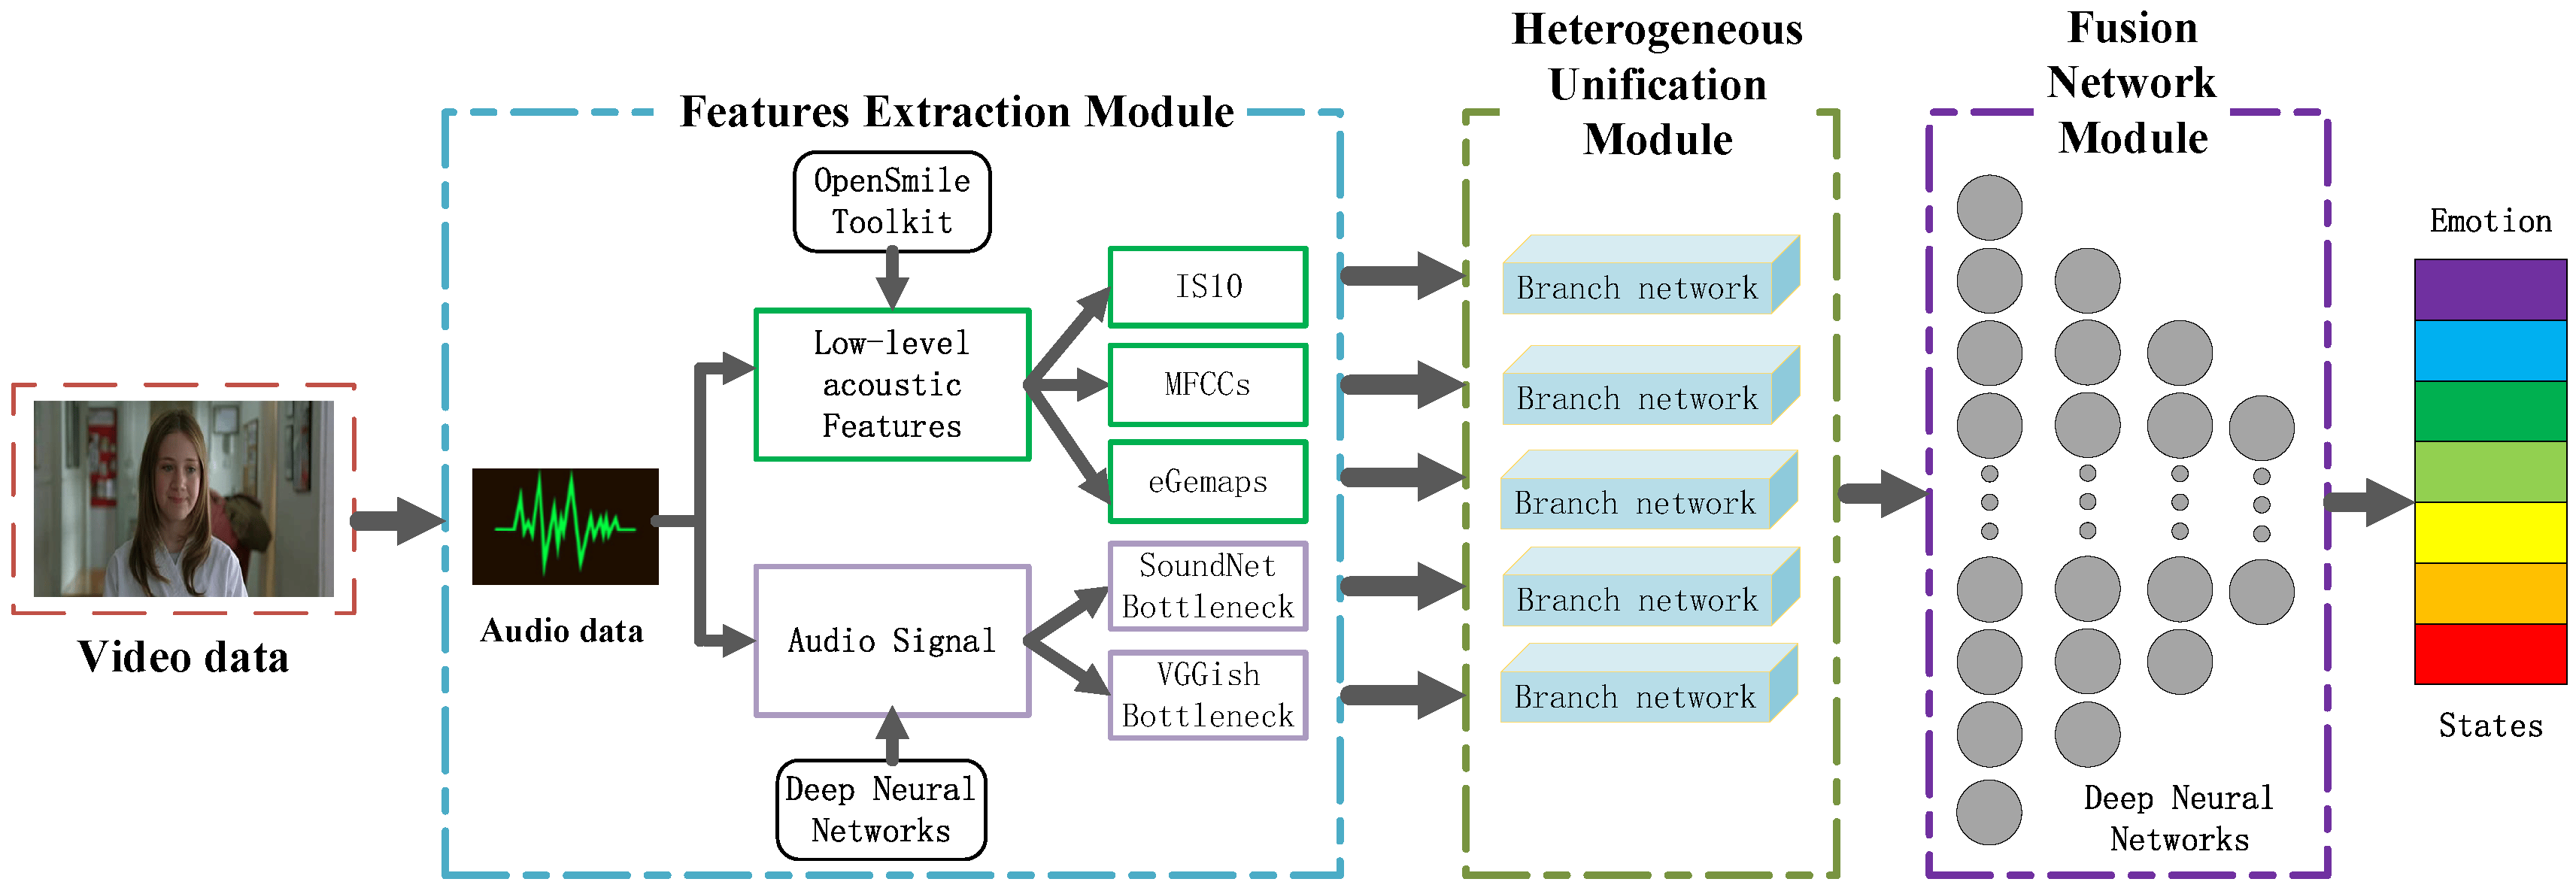
\includegraphics[scale=0.07]{DNN.png}}
\caption{Deep Neural Network architecture for Multimodal emotion detection \cite{s19122730}}
\end{figure}

Francesco Di Luzio et. al \cite{di2023randomized} had proposed the deep learning model  architecture employing parameter randomization in a complex classification model for emotion recognition. 

\section{Conclusion}

Multi modal emotion detection using machine learning is a fast expanding subject, and this overview study provides useful insights into the current state-of-the-art, obstacles, and future research possibilities. As multi modal data becomes more widely available, we anticipate that fusion of information from several modalities will continue to produce promising results, making substantial contributions to real-world applications. A detailed surrey of papers had been taken into consideration which gives the research possibilities in the field of Machine learning with applications on emotion detection. A critical analysis had been done how new techniques can be used to improve the results. 

\bibliographystyle{unsrt}
\bibliography{BibTEXFILE}
\end{document}